\subsection[Architecture  centralisée]{Architecture  centralisée}
\begin{figure}[h]
	\centering
		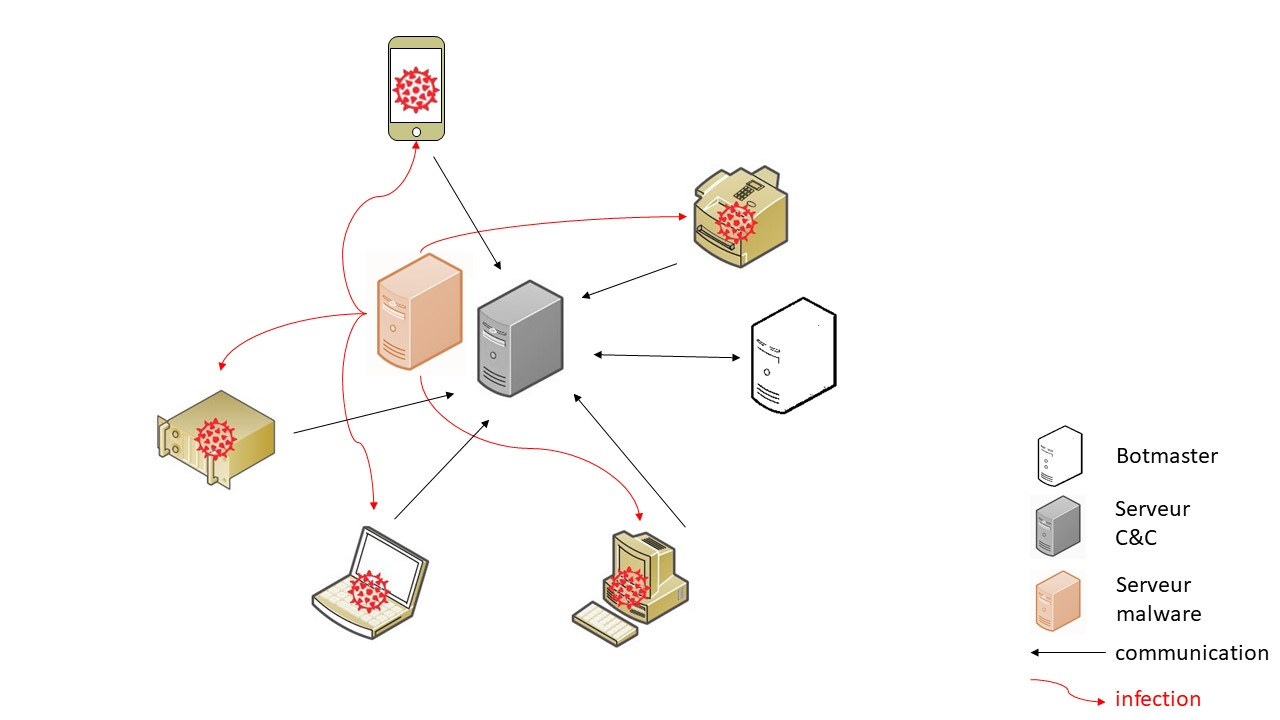
\includegraphics[width=0.75\textwidth]{archi_centralise}
	\label{fig:archicent}
	\caption[Architecture  centralisée]{Architecture  centralisée}
\end{figure}
\begin{figure}[h]
	\centering
		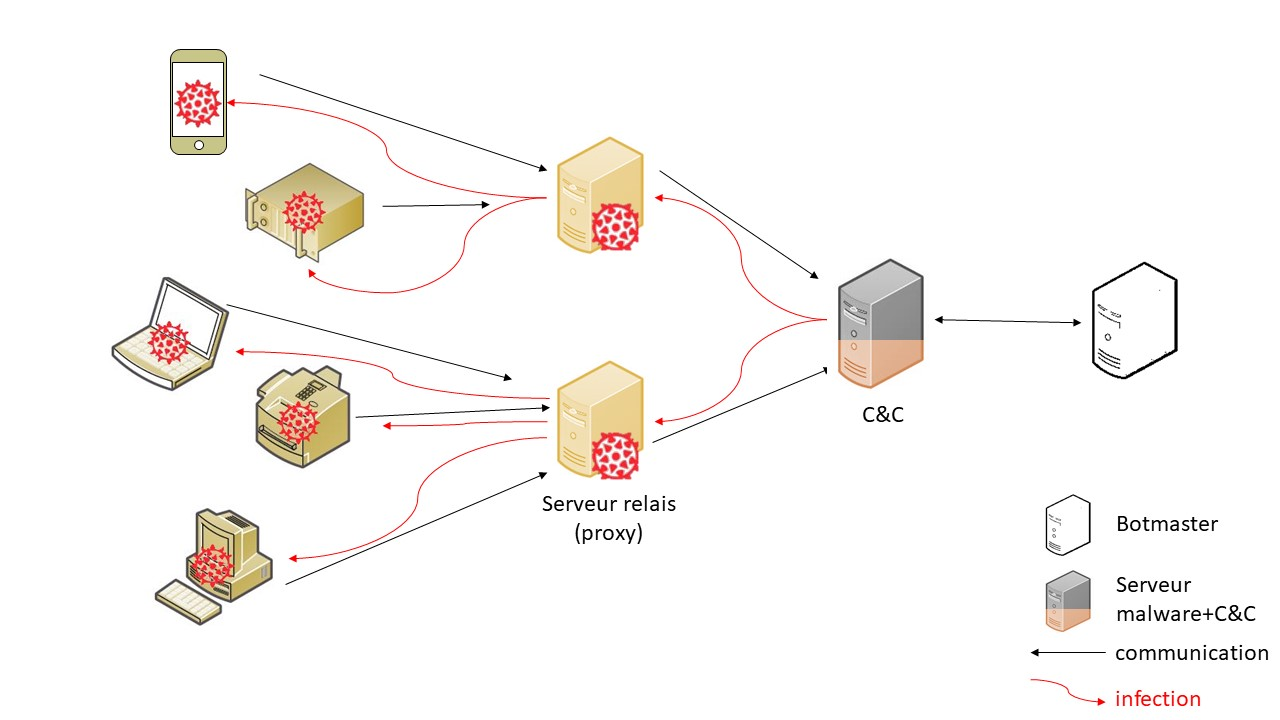
\includegraphics[width=0.75\textwidth]{archi_centralise_2}
	\label{fig:archicent2}
	\caption[Architecture  centralisée répartie par utilisation d’une batterie de serveurs relais]{Architecture  centralisée répartie par utilisation d’une batterie de serveurs relais}
\end{figure}

\subsubsection{Définition}
Un ou plusieurs nœud de communication permettent aux bots d'échanger des données via un canal de communication.
Les nœuds représentent un serveur ou serveur relais avec comme fonction le C\&C.

\subsubsection{Liste des protocoles utilisés par le botnet}
\begin{itemize}
	\item IRC\footnote{Internet Relay Chat}
	\item HTTP\footnote{HyperText Transfer Protocol}
	\item IRC modifié
\end{itemize}

\subsubsection{Avantages}
\begin{itemize}
	\item Architecture  centraliséee
	\item Simplicité de mise en oeuvre (mIRC, ...)
	\item Utilisation des canaux IRC (topics, messages) pour l’envoi des commandes vers les botsPerformance (non gourmant en bande passante)
	\item Connexions régulières entre les bots et le C\&C (non-permanente)
	\item Recherche des ordres dans des forums, avec des mots clés ou même dans des images (stéganographie)
\end{itemize}

\subsubsection{Inconvénients}
\begin{itemize}
	\item Vulnérabilité du botnet (serveur central)
	\item Connexion en permanence
	\item Facile à détecter (filtrage du flux IRC)
\end{itemize}

%--------------------------------------------------------------------
%ajouter un botnet
%glisser le .csv dans le dossier exemples de la section 2
%inclure la ligne \csvautotabular[respect all]{Section/2-Ssection/exemples/nom-du-botnet}
%--------------------------------------------------------------------

\subsubsection{exemples}
\noindent
\resizebox{\textwidth}{!}{
\csvautotabular[respect all]{Section/2-Ssection/exemples/BEBLOH.csv}
}
\noindent
\resizebox{\textwidth}{!}{
\csvautotabular[respect all]{Section/2-Ssection/exemples/BOBAX-KRAKEN.csv}
}